%% Autor: Björn Ritterbecks 
%% Letzte Aenderung: 15.06.2016 
\thisfloatsetup{%
  capbesidewidth=\marginparwidth}
\begin{figure}[htbp]
\vspace*{0.2cm}
\centering
%\sansmath
 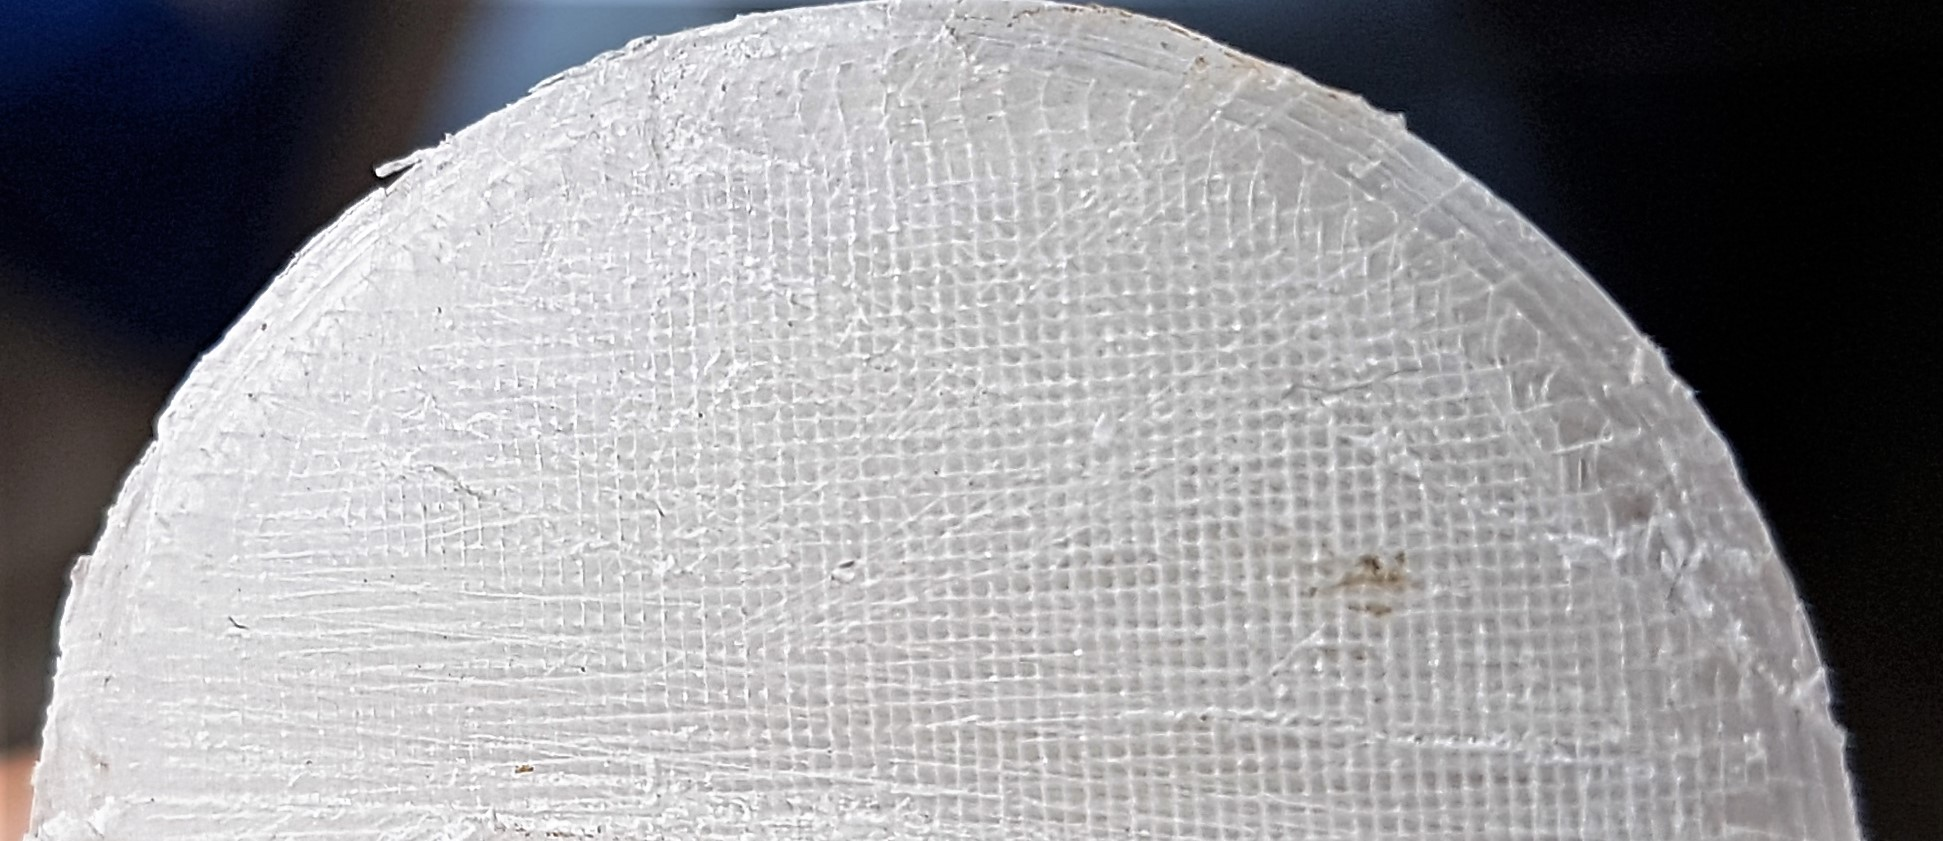
\includegraphics[width=0.99\textwidth]{images/fail.jpg}
  \caption[Aufgeschnittene Kugel aus dem 3D-Drucker]{Auf diesem Foto einer aufgeschnittenen, 3D-gedruckten Kugel ist gut zu erkennen, dass die Wandschicht der Kugel mit einer höheren Dichte gedruckt wurde.}
  \label{fig:fail}
  \vspace{-0pt}
\end{figure}